\chapter{Разработка и экспериментальное внедрение системы радиочастотной идентификации}\label{ch:ch5}
Важная задача, возникающая при построении системы радиочастотной идентификации транспортных средств "--- необходимость объединять в реальном времени данные со множества считывателей, которые могут быть размещены на большой территории. Для решения этой задачи была разработана распределенная платформа для интеграции и управления RFID-считывателями. Платформа позволяет интегрировать разрозненные считыватели в единую масштабируемую систему обработки данных.

В 2014--2015 годах был проведён эксперимент в городе Казань, в ходе которого было проведено испытание разработанной платформы и RFID-считывателей для идентификации меток, размещённых на рейсовых автобусах. Весной 2020 года в рамках НИР были проведены протокольные испытания на полигоне в городе Казань для проверки системы при идентификации меток на автомобилях, движущихся со скоростями до 160~км/ч. Все испытания завершились успешно.

В этой главе приводится описание разработанной платформы и проведённого эксперимента, обсуждаются его результаты. В разделе \ref{sec:ch5_architecture} описывается структура платформы управления считывателями и её основные компоненты, в разделе \ref{sec:ch5_protocols} "--- разработанные протоколы, а в разеделе \ref{sec:ch5_applications} "--- приложения, которые могут работать в составе системы. Далее, в разделе \ref{sec:ch5_implementation}, описывается реализация платформы, использованная в эксперименте в городе Казань. В разделе \ref{sec:ch5_results} приводятся результаты, полученные в ходе эксперимента, а также приводятся некоторые наблюдения, отмеченные при проведении эксперимента. Раздел \ref{sec:ch5_conclusion} завершает главу.

Результаты, представленные в главе, были опубликованы в работах, индексируемых Scoupus/WoS \cite{RFIDCTRL_NETS2CARS2014, RFIDTA2012}, и представлены в трудах конференций \cite{RFIDCTRL_DCCN2017, RFIDCTRL_VSPU2014}. По результатам эксперимента 2020 года был сделан доклад на форуме Kazan Digital Week 2020.


%%%%%%%%%%%%%%%%%%%%%%%%%%%%%%%%%%%%%%%%%%%%%%%%%%%%%%%%%%%%%%%%%%%%%%%%%%%%%%%%
\section{Архитектура системы управления считывателями}\label{sec:ch5_architecture}
%%%%%%%%%%%%%%%%%%%%%%%%%%%%%%%%%%%%%%%%%%%%%%%%%%%%%%%%%%%%%%%%%%%%%%%%%%%%%%%%
Радиочастотная идентификация транспорта может применяться для идентификации автомобилей в системах регистрации нарушений правил дорожного движения, для оплаты проезда по платным дорогам, доступа на закрытые территории, а также использоваться при поиске угнанных машин и розыске преступников. Для быстрой реализации различных приложений программное обеспечение должно предоставлять возможность быстрого добавления новых сервисов в систему, а также обеспечивать масштабируемость.

\begin{figure}[ht]
  \centerfloat{
    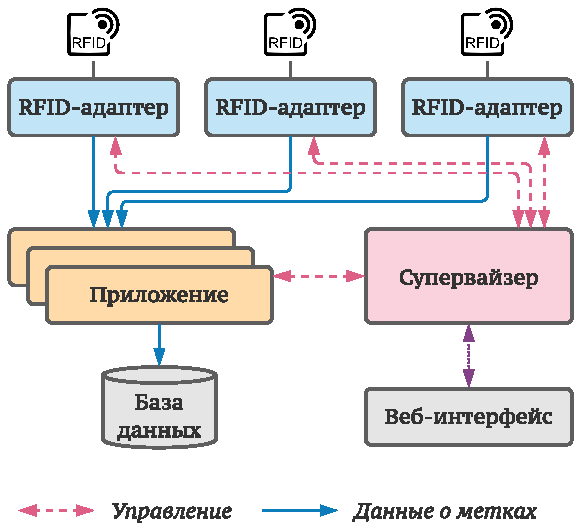
\includegraphics [width=0.5\textwidth]{chapter5/ch5_components}
  }
  \caption{Компоненты системы управления}
  \label{fig:ch5_components}
\end{figure}

Система управления считывателями имеет модульную структуру (см. рис.~\ref{fig:ch5_components}) и включает три типа модулей: супервайзеры, RFID-адаптеры и приложения. Супервайзеры (SVR) отвечают за хранение и управление конфигурацией системы. RFID-адаптеры управляют работой радиомодулей RFID-считывателей, реализуют чтение и запись меток. Приложения обрабатывают потоки прочитанных меток, поступающих от RFID-адаптеров и других приложений. Приложения могут использоваться для объединения потоков от нескольких источников, фильтрации или преобразования протоколов. Кроме перечисленных модулей, в состав системы входят иструменты администрирования "--- консоль и веб-интерфейс.

Каждый модуль системы поддерживает множество объектов, каждый из которых является либо параметром, либо процедурой. Обработка объектов ведётся по запросам, приходящим от пользователей или других модулей системы. Множество объектов полностью определяется типом модуля. Например, каждый RFID--адаптер поддерживает параметры <<температура радио--модуля>>, <<значение Q>>, <<номер сессии>> и процедуры <<выключить радио--модуль>>, <<включить радио--модуль>>. RFID--адаптер, специализированный на поддержке определенного считывателя, может предоставлять объекты, специфичные для конкретной модели считывателя. Каждый модуль получает свои настройки от супервайзера сразу после включения.

Для работы с объектом пользователь или модуль должны отправить запрос супервайзеру через один из поддерживаемых им протоколов управления (рассматриваются ниже). Супервайзер поддерживает множество собственных объектов, например "--- <<число активных пользователей>> или <<статус подключений модулей>>, а также выполняет проксирование объектов всех подключенных модулей. Когда супервайзер получает запрос на объект, который не принадлежит ему самому, он перенаправляет запрос модулю, которому этот объект принадлежит, и отвечает клиенту, перенаправляя ответ, полученный от модуля.

В системе используется разделение потоков данных и управления: все управление производится через супервайзер, а данные передаются напрямую между RFID-адаптерами и приложениями. Такое разделение позволяет, с одной стороны, снизить нагрузку на супервайзер и увеличить масштабируемость, а с другой "--- использовать более простые протоколы между компонентами. Так как основное назначение системы "--- непрерывное чтение меток проезжающих автомобилей, передача данных о прочитанных метках организована в виде потоков. Приложение, которое хочет получать данные о метках от RFID-адаптера или другого приложения должно подписаться подписаться на поток.

Пользователи могут настраивать систему и взаимодействовать с RFID-адаптерами и приложениями. В системе определены четыре уровня доступа: наблюдатели, операторы, администраторы и суперпользователи. Наблюдатели могут подписываться на потоки меток, но не могут записывать метки или менять настройки оборудования. Операторы имеют право настраивать RFID--адаптеры и выполнять операции чтения/записи меток, но не могут менять настройки остальных компонентов системы. Администраторы имеют право настраивать модули, но не могут записывать метки. Суперпользователи имеют права на любые действия с системой. Помимо уровней доступа пользователей с каждым компонентом связан специальный системный уровень доступа, который позволяет ему работать с определенным набором объектов других компонентов. Например, приложения могут читать, но не имеют права записывать параметры RFID--адаптеров.

Поскольку все модули системы взаимодействуют друг с другом по сети, физически они могут располагаться где угодно. Типичные примеры размещений модулей показаны на рис.~\ref{fig:ch5_deployments}.

\begin{figure}[ht]
  \centerfloat{
    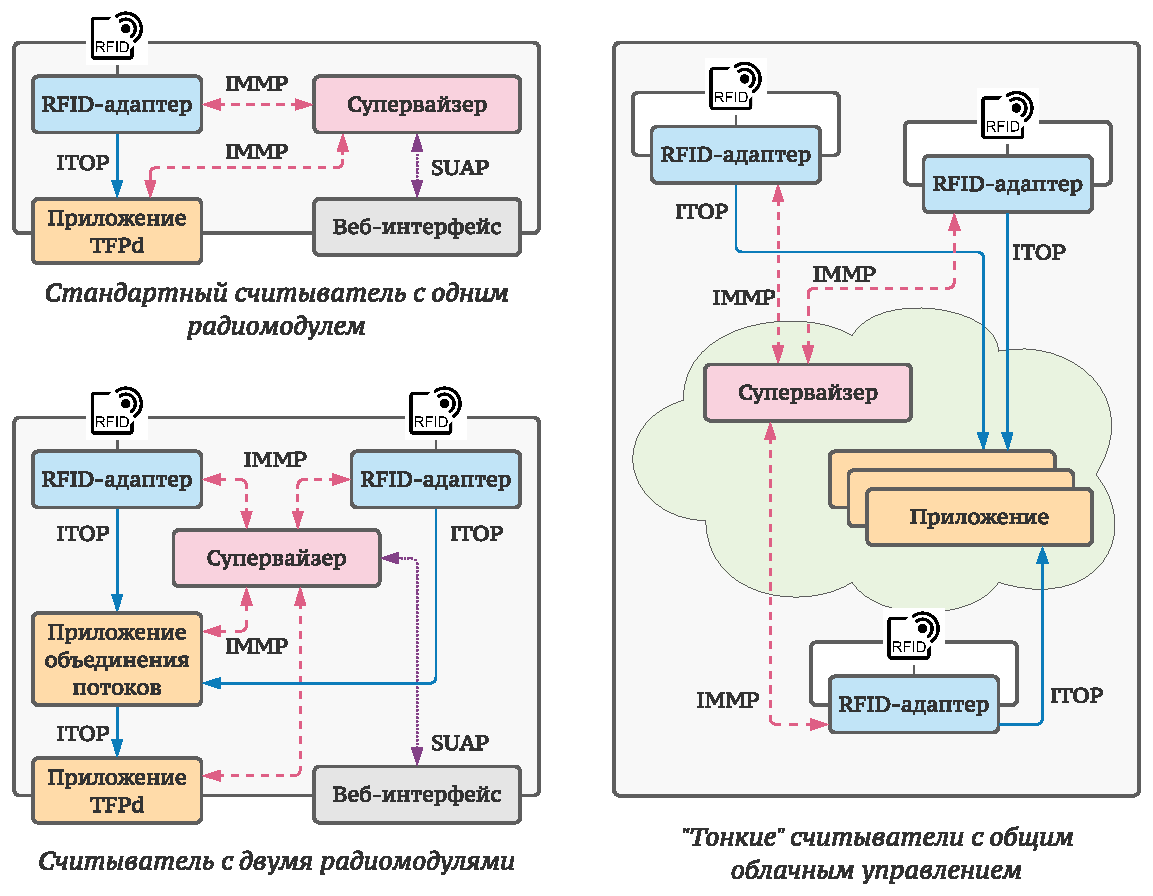
\includegraphics [width=0.9\textwidth]{chapter5/ch5_deployments}
  }
  \caption{Примеры размещения модулей системы}
  \label{fig:ch5_deployments}
\end{figure}

Для обычного RFID--считывателя, построенного на базе среднего процессора (например, одноядерный ARM A7 или ARM A8), обладающего небольшим объемом оперативной памяти порядка 256--512~МБ и имеющего в составе один радиомодуль, достаточно установить супервайзер, RFID-адаптер, а также приложение для подключения к потоку прочитанных меток снаружи (TFPd) и модуль, предоставляющий доступ к настройке считывателя через веб-интерфейс или консоль. Такое размещение компонентов позволяет передавать данные обо всех прочитанных метках в центр обработки данных и, при необходимости, реализовывать операции чтения/записи через подключение внешних модулей и пользователей. Именно такая конфигурация считывателей использовалась во всех проведенных экспериментах.

Если считыватель имеет более мощное вычислительное ядро, на нём можно разместить несколько приложений. Например, на нем можно установить приложения для фильтрации прочитанных меток или нахождения соответствий с номерными знаками, распознанными камерами. Если считыватель включает несколько радиомодулей, то потребуется несольких RFID--адаптеров. Хотя каждый компонент системы не требователен к вычислительным ресурсам по отдельности, для выполнения задач обработки потоков меток могут потребоваться дополнительные ресурсы. Желательно использовать 2-х или 4-х ядерный процессор ARM и 512 "--- 1024 МБ оперативной памяти.

В наиболее сложном случае система может работать в распределенном режиме, а различные ее компоненты размещаться на считывателях и серверах, при этом считыватели могут быть сделаны чрезвычайно <<тонкими>> "--- на них достаточно разместить RFID--адаптер, который будет подключаться по сети к супервайзеру, работающему на внешнем сервере или в облаке. Приложения также могут работать на отдельных физических или виртуальных внешних серверах. В этом варианте считыватели могут быть реализованы на самых простых вычислительных компонентах, что позволит снизить их стоимость, а приложения и супервайзер выполняются в центре обработки данных на мощном вычислительном оборудовании, благодаря чему им можно поручить работу с большим числом считывателей. Такой вариант размещения наиболее гибок и позволяет построить распределенную систему, состоящую из сотен считывателей, каждый из которых может администрироваться из единой консоли.



%%%%%%%%%%%%%%%%%%%%%%%%%%%%%%%%%%%%%%%%%%%%%%%%%%%%%%%%%%%%%%%%%%%%%%%%%%%%%%%%
\section{Протоколы взаимодействия компонентов системы}\label{sec:ch5_protocols}
%%%%%%%%%%%%%%%%%%%%%%%%%%%%%%%%%%%%%%%%%%%%%%%%%%%%%%%%%%%%%%%%%%%%%%%%%%%%%%%%

В системе управления передача данных и управления разделены. Для упрвления системой были разработаны протоколы IMMP (Internal Modules Management Protocol) и SUAP (Simple User Access Protocol), а для передачи потоков меток и работы с радиомодулями "--- протоколы ITOP (Internal Tags Operation Protocol) и TFP (Tag Flow Protocol). Протоколы IMMP и ITOP используются для управления и передачи внутри системы, а протоколы SUAP и TFP "--- для работы работы с супервайзером со стороны интерфейсов управления и получения потоков прочитанных меток во внешние информационные системы. Все протоколы, используемые в системе, показаны на рис.~\ref{fig:ch5_protocols}.

\begin{figure}[ht]
  \centerfloat{
    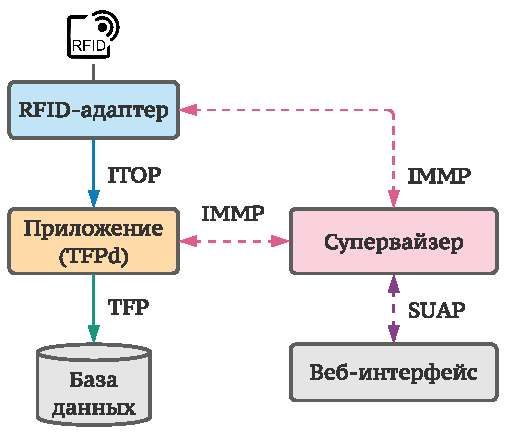
\includegraphics [width=0.5\textwidth]{chapter5/ch5_protocols}
  }
  \caption{Протоколы передачи данных и управления.}
  \label{fig:ch5_protocols}
\end{figure}

Все протоколы имеют клиент--серверную архитектуру, соединение создаётся клиентом. Каждый запрос должен подтверждаться получателем с помощью специального сообщения Response, содержащего результат обработки запроса или код ошибки. Запросы упорядочиваются с помощью порядкового номера ReqSN (Request Sequence Number): клиент и сервер поддерживают счетчики, перед отправкой значение счетчика увеличивается и помещается в соответствующее поле в запросе. В ответе на запрос поле ReqSN должно совпадать со значением счетчика из запроса. Этот механизм позволяет реализовать асинхронную обработку запросов "--- отправителю запроса не нужно ждать ответа для того, чтобы передать новый запрос. При этом отправитель может быть уверен, что запросы будут обработаны в порядке их передачи: если получатель видит, что номер запроса меньше последнего обработанного, запрос будет проигнорирован. С каждым запросом также связано максимальное ожидание ответа, после которого отправитель считает, что запрос не был выполнен.

Формат сообщений, кодируемых с помощью ASCII-строк, аналогичен форматам, используемым в HTTP v1.1 и SIP.


%%% --------------------------------------------
\subsection{IMMP "--- протокол управления модулями}\label{sec:ch5_immp}
%%% --------------------------------------------

Протокол IMMP работает поверх транспортного уровня TCP и реализует функции получения модулями своей начальной конфигурации от супервайзера, поиск IP-адреса модуля по имени (сервис локации), получение и установка значений объектов, а также удалённый вызов процедур. В роли сервера всегда выступает супервайзер, а клиента "--- один из модулей системы.

В протоколе определены семь запросов: HELLO, ACK, BYE, GET, SET и CALL. Запрос HELLO отправляется клиентом для создания соединения. Если соединение может быть установлено, сервер (супервайзер) сначала передает ответ с кодом успеха (200), а затем "--- запрос ACK, в котором супервайзер передает конфигурацию модуля и ключ сессии (SKey, Session Key). Запросы GET и SET используются для чтения и записи значений объектов--параметров, а запрос CALL "--- для удаленного вызова процедур. Запросы GET, SET и CALL могут передаваться как клиентом, так и сервером.

\begin{figure}[ht]
  \centering
  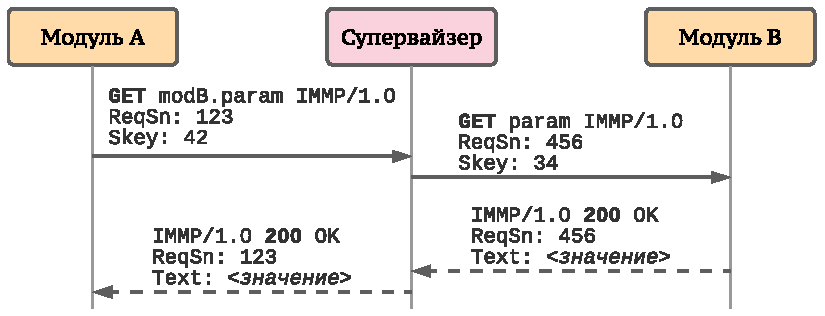
\includegraphics [width=0.75\textwidth] {chapter5/ch5_immp_proxy}
  \caption{Работа супервайзера в режиме IMMP-прокси.}
  \label{fig:ch5_immp_proxy}
\end{figure}

Если супервайзеру нужно выполнить какую-либо операцию над объектом другого модуля, он передает соответствующий запрос (GET, SET или CALL). Если же модулю A нужно выполнить действие над объектом модуля B, то супервайзер выступает в роли прокси-сервера: модуль A передает запрос супервайзеру, который тот передает модулю B, дожидается ответа и пересылает его обратно модулю A (см. рис.~\ref{fig:ch5_immp_proxy}).

\begin{figure}[ht]
  \centering
  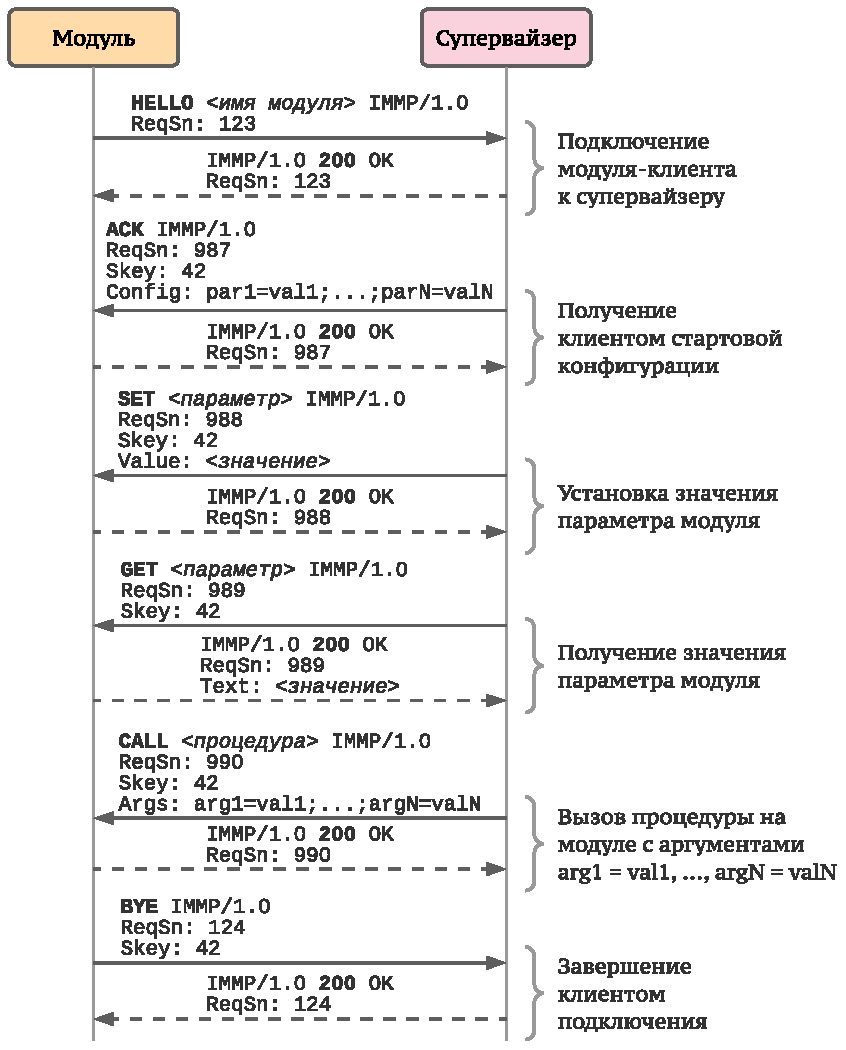
\includegraphics [width=0.85\textwidth] {chapter5/ch5_immp_session}
  \caption{Пример IMMP-сессии}
  \label{fig:ch5_immp_session}
\end{figure}

Пример соединения показан на рис.~\ref{fig:ch5_immp_session}. Клиент передает запрос HELLO со своим именем, сервер отвечает кодом 200. Затем супервайзер готовит стартовую конфигурацию клиента и передает ее в запросе ACK, получение которого клиент должен подтвердить. Такое разделение ответов сервера возникает из-за того, что при высокой нагрузке на супервайзер подготовка стартовой конфигурации может занять время, которое может превышать время ожидания ответа на запрос HELLO. После получения ответа на HELLO клиент может ждать гораздо дольше получения своей конфигурации в ACK. Помимо начальной конфигурации, в ACK супервайзер передает ключ сессии SKey, который используется в дальнейшем обмене сообщениями. После обмена запросами HELLO и ACK начинается основная часть сессии. В ней клиент и сервер обмениваются запросами GET, SET и CALL. Завершает сессию в этом примере клиент отправкой запроса BYE.



%%% --------------------------------------------
\subsection{SUAP "--- протокол подключения интерфейсов управления}\label{sec:ch5_suap}
%%% --------------------------------------------

Протокол SUAP представляет собой упрощенную версию IMMP, работающую через UDP. Он предназначен для подключения пользовательских интерфейсов к супервайзеру. В функции SUAP входят получение и установка значений параметров, удаленный вызов процедур и обнаружение компонентов. Предполагается, что модули, предоставляющие пользователям доступ, не имеют своих объектов, поэтому передавать им начальную конфигурацию не надо, соответственно, отсутствует запрос ACK. По этой же причине протокол не является симметричным "--- запросы GET, SET и CALL могут передаваться только от клиента серверу. Кроме этого, есть некоторые отличия в кодировании ответов: если в IMMP значение параметра в ответе на запрос GET передается в поле заголовка Text, то в SUAP значение параметра содержится в теле ответа, отделенном пустой строкой от последнего заголовка.

\begin{figure}[ht]
  \centering
  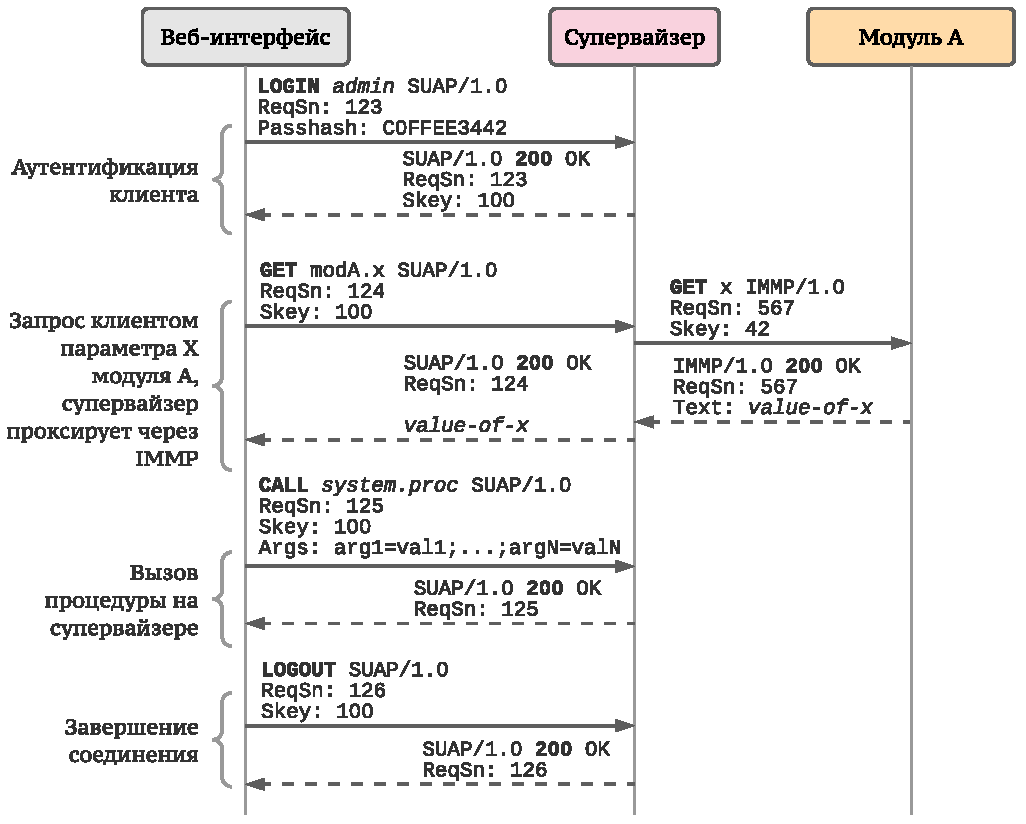
\includegraphics [width=0.95\textwidth] {chapter5/ch5_suap_session}
  \caption{Пример SUAP-сессии}
  \label{fig:ch5_suap_session}
\end{figure}

Аутентификация пользователей производится с помощью логина и пароля. Пароль может передаваться либо нешифрованным текстом, либо в виде хеша. В отличие от IMMP, вместо запроса HELLO клиент в начале сессии должен отправить запрос LOGIN, а для заврешения сессии "--- запрос LOGOUT. Ключ сессии (SKey) используется для авторизации запросов клиента и передается супервайзером в ответе на запрос LOGIN. Пример сессии SUAP показан на рис.~\ref{fig:ch5_suap_session}.

Отметим, что использование SKey для авторизации запросов не является безопасным: если злоумышленник сможет перехватить UDP-пакеты SUAP-сессии, то он сможет получить и использование значение SKey вместо клиента. Вопросы обеспечения защиты информации в системе управления требуют дальнейшей разработки, возможные решения "--- использование шифрования DTLS (Datagram Transport Layer Security) или замена SUAP на HTTPS и реализация REST API на супервайзере.



%%% --------------------------------------------
\subsection{Протокол работы с RFID-адаптерами (ITOP)}\label{sec:ch5_itop}
%%% --------------------------------------------

Протокол предназначен для связи между компонентами системы (приложениями и RFID-адаптерами), желающими осуществлять действия над метками. Он позволяет читать и записывать память меток, а также подписываться на потоки считанных меток. Подписка может быть позднее отменена, также она завершается при закрытии соединения любой из сторон.

В протоколе определены семь запросов: HELLO, BYE, READMEM, WRITEMEM, WRITEEPC, SUBSCRIBE, UNSUBSCRIBE. Сервер может передать запрос BYE, остальные запросы передаются только клиентом. Запросы HELLO и BYE используются для создания и завершения соединений. SUBSCRIBE и UNSUBSCRIBE используются для создания и отмены подписки, а запросы READMEM, WRITEMEM и WRITEEPC "--- для чтения или записи данных на заданную метку.

В протоколе ITOP также определен специальный вид сообщения--ответа NOTIFY. Это сообщение асинхронно передаётся сервером для информирования клиента, подписавшегося на поток, о прочтении новой метки. Тело сообщения может содержать следующие поля:

\begin{itemize}
	\item epc: значение EPC прочитанной метки;
	\item tid: значение банка TID прочитанной метки;
	\item power: мощность принятого сигнала;
	\item antenna: номер антенны, на которой была считана метка;
	\item frequency: частота, на которой работал считыватель;
	\item count: число раз, которое метка была считана;
	\item um: содержимое банка памяти USER MEMORY;
	\item source: имя RFID--адаптера, считавшего метку;
	\item id: идентификатор метки.
\end{itemize}

Поле id может заполняться данными, специфичными для приложения, например "--- значением EPC или номером транспортного средства, полученным приложением с помощью обращения к базе данных. Поле um используется только при чтении банка пользовательской памяти, а поле source нужно только при использовании нескольких RFID-адаптеров. Если какие-то из полей не содержат данных, их можно опустить. Значение каждого поля передается в отдельной строке, общее число строк содержится в заголовке Content-length.

Когда клиент хочет установить ITOP-соединение, он передает серверу запрос \texttt{HELLO}. В этот запрос клиент включает значение \texttt{SKey}, полученное ранее при создании IMMP- или SUAP--соединения. Значение \texttt{SKey} используется для авторизации сервером клиента на выполнение той или иной операции. Например, администраторы и наблюдатели не имеют права записывать метки, а единственная разрешенная им операция "--- создание подписки на получение потока меток.

% \begin{figure}[ht]
%   \centerfloat{
%     \includegraphics [width=0.8\textwidth] {chapter5/ch5_itop_session}
%   }
%   \legend{Клиент подключается по IMMP к SVR и получает ключ сессии \texttt{SKey}, затем запрашивает адрес ITOP-сервера. Получив адрес, клиент создает соединение с ITOP-сервером с использованием ключа \texttt{SKey}, создает подписку на получение меток. После получения двух меток клиент отменяет подписку и завершает соединение.}
%   \caption{Пример ITOP-сессии}
%   \label{fig:ch5_itop_session}
% \end{figure}

Если клиент желает непрерывно получать информацию о прочитанных метках от сервера, он передает запрос SUBSCRIBE. Как только считывается (если сервер "--- RFID-адаптер) или принимается (если сервер "--- приложение) новая метка, сервер передает сообщение NOTIFY клиенту, содержащее информацию о метке. Когда клиент желает остановить получение потока, он отменяет подписку передачей запроса UNSUBSCRIBE.

Пример сессии с показан на рис.~\ref{fig:ch5_itop_session}


%%% --------------------------------------------
\subsection{Протокол потокового чтения меток (TFP)}\label{sec:ch5_tfp}
%%% --------------------------------------------

Протокол TFP является упрощенной версией протокола ITOP и предназначен для получения данных о метках из пользовательских интерфейсов или внешних клиентов. Специальное приложение TFP Daemon (TFPd) реализует TFP-интерфейс и выступает в роли моста между ITOP и TFP: с одной стороны это приложение выступает в роли сервера протокола TFP, с другой "--- клиента ITOP. В протоколе TFP поддерживается только механизм создания подписок, прочие функции (запись меток, чтение заданных областей памяти и пр.) он не реализует. Кроме того, в сообщении \texttt{HELLO} не передается ключ сессии \texttt{SKey}, так как приложение TFPd использует свой собственный (системный) уровень доступа для создания ITOP-соединения с источником данных, позволяющий создавать подписки.



%%%%%%%%%%%%%%%%%%%%%%%%%%%%%%%%%%%%%%%%%%%%%%%%%%%%%%%%%%%%%%%%%%%%%%%%%%%%%%%%
\section{Приложения в программной платформе}\label{sec:ch5_applications}
%%%%%%%%%%%%%%%%%%%%%%%%%%%%%%%%%%%%%%%%%%%%%%%%%%%%%%%%%%%%%%%%%%%%%%%%%%%%%%%%

Кратко рассмотрим основные приложения, использующиеся в системе: агрегатор потоков AggrApp и TFP-сервер TFPd и кэш CacheApp. Работа этих приложений показана на рис.~\ref{fig:ch5_applications_scheme}.

В дальнейшем могут быть реализованы более сложные приложения: фильтрация и модификация потока меток, преобразование протоколов (например, для подключения к платформе по протоколу web sockets), поиск номеров автомобилей по меткам в реальном времени и прочие.


%%% --------------------------------------------
\subsection{Агрегация потоков (AggrApp)}
%%% --------------------------------------------

Большинство приложений может подключаться к единственному ITOP-потоку. Если нужно объединить данные, поступающие от двух или более источников данных, можно использовать приложение AggrApp. Его функция "--- пересылка всем клиентам каждого \texttt{NOTIFY}-сообщения, поступающего в любом из входящих ITOP-соединений. Это единственное из приложений, имеющих множественный вход и множественный выход.

Приложение AggrApp создает подписки у своих источников данных только тогда, когда к нему подключается и создает подписку первый клиент. Если ни один клиент не подписан на поток от приложения, само приложение также не инициирует подписку.


%%% --------------------------------------------
\subsection{TFP-сервер и кэш}
%%% --------------------------------------------

Компоненты внутри системы используют протокол ITOP для чтения и записи меток. В то же время, для подключения внешних клиентов (например, для записи данных о проездах в базу данных в центре обработки данных) не нужны все функции ITOP. В частности, не нужно (и даже не желательно) иметь возможность записывать метки из ЦОДа. Для упрощения таких задач используется протокол TFP, который был рассмотрен ранее "--- в отличие от ITOP, он предоставляет возможность только для управления подпиской на поток данных о прочитанных метках.

Для того, чтобы преобразовать поток данных о прочитанных метках, получаемый от адаптеров или других приложений по протоколу ITOP, в TFP-поток, применяется приложение TFPd. При подключении первого клиента и создания этим клиентом подписки, TFPd связывается с источником данных по протоколу ITOP, подписывается на ITOP-поток и передает все \texttt{NOTIFY}-сообщения из ITOP-сессии в TFP-сессии. При отлючении последнего TFP-клиента подписка на ITOP-поток также отменяется.

Еще одно приложение, CacheApp, размещается обычно на том же оборудовании, на котором работает TFPd, и сохраняет в файл журнала все данные, полученные от него по протоколу TFP. Это приложение оказывается особенно полезным, когда и RFID-адаптер, и TFP-сервер расположены на считывателе, который связан с центром обработки данных плохим каналом связи и позволяет избежать потери данных о прочитанных метках.



%%%%%%%%%%%%%%%%%%%%%%%%%%%%%%%%%%%%%%%%%%%%%%%%%%%%%%%%%%%%%%%%%%%%%%%%%%%%%%%%
\section{Экспериментальная реализация системы}\label{sec:ch5_implementation}
%%%%%%%%%%%%%%%%%%%%%%%%%%%%%%%%%%%%%%%%%%%%%%%%%%%%%%%%%%%%%%%%%%%%%%%%%%%%%%%%

Все описанные программные модули и протоколы, кроме части RFID-адаптера, взаимодействующей со считывателем и веб-интерфейса, были реализованы на языке C++. Часть RFID-адаптера, работающая непосредственно с радиомодулем считывателя, была реализована на C. Для реализации web-интерфейса использовался фреймворк Flask на языке Python 3. Все компоненты системы работают под управлением операционной системы Linux.

Помимо перечисленных ранее, в системе присутствует специальное приложение (RRRd), осуществляющее запуск и остановку компонентов.

Следует выделить несколько особенностей, общих для всех модулей кроме веб-интерфейса, реализованного на Python. Во-первых, в реализациях очередей, клиентов и серверов практически не используется динамическая память (функции \texttt{malloc}/\texttt{free}, операторы \texttt{new}/\texttt{delete} и пр.). Вместо этого под каждое сообщение или очередь заранее статически выделяется область памяти, заведомо превышающая предельно допустимый размер хранимого объекта. Этот подход позволяет не только повысить производительность за счёт отсутствия работы с выделением и освобождением памяти, но и существенно повысить надёжность за счёт снижения вероятности появления ошибок утечки памяти или обращений к ранее освобождённой памяти.

Во-вторых, большинство модулей, включающих серверы каких либо протоколов (IMMP, ITOP и пр.) имеют в своем составе очереди, с помощью которых обработка запросов от различных клиентов мультиплексируется и может осуществляться даже одним потоком. Опрос сокетов также производится мультиплексированием функцией \texttt{pselect}. Более подробно эта идея будет описана на примерах SVR и RFID-адаптеров далее.

В-третьих, все модули реализованы в виде многопоточных приложений с использованием библиотеки pthreads (POSIX Threads).

Наибольшую сложность при разработке системы представляли супервайзер (SVR) и RFID-адаптер, поэтому в следующих разделах они рассмотрены подробнее.



%%% --------------------------------------------
\subsection{Реализация супервайзера}
%%% --------------------------------------------

В состав SVR входит очередь (управляется отдельным потоком), множество потоков-рабочих и поток-сервер.

\textbf{Поток-сервер} осуществляет запуск и остановку других потоков, взаимодействует с RRRd, а также выполняет роль сервера протоколов SUAP и IMMP. При запуске он открывает серверные сокеты протоколов SUAP и IMMP, создаёт TCP-сессии протокола IMMP по мере поступления запросов на соединения. Опрос сокетов производится методом мультиплексирования с помощью функции \texttt{pselect}. При получении сообщения протокола SUAP или IMMP поток-сервер создаёт событие и записывает его в очередь.

\textbf{Поток управления очередью} осуществляет помещение и извлечение событий из очереди, а также отслеживает директивные сроки каждого события. При истечении срока события оно извлекается из очереди, а в сессии IMMP или клиенту SUAP передается ответ с кодом ошибки, соответствующему истечению времени ожидания. Это позволяет своевременно оповещать клиентов о перегрузке системы и не тратить вычислительные ресурсы на обработку событий, которые с большой вероятностью уже не актуальны для клиента.

\textbf{Потоки-рабочие} осуществляют обработку событий. Например, если в событии содержится запрос на получение значения объекта, хранимого в другом модуле, рабочий произведёт обращение по протоколу IMMP к соответствующему модулю и, получив ответ, передаст его тому модулю, который инициировал запрос. Количество рабочих настраивается и, в зависимости от того, сколько модулей обслуживает SVR, может меняться от 1-2 до 10 и более, тем самым обеспечивая масштабирование системы в зависимости от нагрузки, а также используемой аппаратной платформы. Следует отметить, что слишком мало потоков-рабочих не следует делать даже на одноядерных системах, поскольку при обработке запросов им часто приходится ожидать ответов в течение времени, превышающего время активной обработки события.


%%% --------------------------------------------
\subsection{Реализация адаптера RFID}
%%% --------------------------------------------

Особенностью этого модуля является необходимость использования программного интерфейса радиомодуля, написанного на языке C. Для того, чтобы иметь возможность быстрой замены модулей, была реализована промежуточная библиотека (также на языке C), реализующая основные функции: чтение метки в течение заданного временного интервала, запись значение EPCID на метку, запись значения в заданный банк памяти, получение и запись значения параметра модуля.

Хотя дизайн промежуточной библиотеки был сделан очень близким к операциям, предоставляемым API использованного радиомодуля, её несложно адаптировать к радиомодулям других производителей, при наличии соответствующей спецификации протокола взаимодействия или API.

Сам протокол ITOP предоставляет два вида операций чтения: потоковое и по запросу. Поскольку одновременно к адаптеру могут подключаться несколько модулей (например, TFPd и веб-интерфейс), нужно обеспечить мультиплексирование доступа к радиомодулю, играющего роль разделяемого ресурса, причём должен обеспечиваться доступ для одновременного потокового чтения и чтения по запросу. К тому же, необходимо обеспечить возможность настройки параметров радиомодуля даже в то время, когда он занят чтением меток. Для решения этой задачи в RFID-адаптере была построена \textbf{очередь событий}, которая заполнялась событиями в зависимости от наличия подписок и пришедших запросов по ITOP- или IMMP-соединениям. Всего было определено четыре основных события: чтение меток в течение интервала $T$, запись значения на метку, получение и установка значения параметра;

Каждое событие имеет приоритет, причём для операции чтения он самый низкий. Важной общей чертой всех событий является то, что их обработка требует ограниченного времени, то есть никакое из событий не может захватить адаптер на неопределённо долгий срок.

Если хотя бы один клиент по протоколу ITOP запросил потоковое чтение, то в очередь добавляется событие чтения. По его завершению данные о прочитанных метках передаются всем клиентам, запросившим чтение меток (как потоковое, так и не потоковое), а в очередь добавляется новое событие чтения с тем же интервалом времени. Если другой клиент запрашивал чтение в течение времени, большего используемого интервала $T$, или хотел прочесть дополнительные банки памяти, то вместо очереднго события чтения добавляется новое, содержащее параметры этого запроса.

Если приходит запрос на получение или изменение параметра адаптера, или же на запись данных на метку, то для них создаются соответствующие события. Так как эти события имеют приоритет выше, чем чтение, то они выполнятся раньше, независимо от наличия запросов на потокове или обычное чтение. Как следствие, супервайзеру, как и другим модулям, требуется меньше потоков: в текущей модели все TCP-сессии постоянны, а передача запроса и получение ответа происходят синхронно, то есть рабочий ждет ответа на переданный запрос. Если бы операции чтения меток вытесняли операции чтения или записи параметров, рабочие потоки SVR были бы вынуждены подолгу ждать ответа, что неизбежно сказалось бы на работоспособности и масштабируемости всей системы.

Когда все клиенты, ранее подписавшиеся на получение данных о прочитанных метках в потоке, завершают свою подписку или отключаются, автоматическое добавление новых событий чтения также прекращается. Таким образом, при отсутствии модулей, подписанных на чтение меток, радиомодуль не используется, что, в частности, позволяет снизить энергопотребление и температуру считывателя.



%%%%%%%%%%%%%%%%%%%%%%%%%%%%%%%%%%%%%%%%%%%%%%%%%%%%%%%%%%%%%%%%%%%%%%%%%%%%%%%%
\section{Результаты эксперимента и их анализ}\label{sec:ch5_results}
%%%%%%%%%%%%%%%%%%%%%%%%%%%%%%%%%%%%%%%%%%%%%%%%%%%%%%%%%%%%%%%%%%%%%%%%%%%%%%%%

В конце осени 2014 года был запущен большой эксперимент в городе Казани (республика Татарстан). В ходе эксперимента номерами с радиометками были оснащены 740 автобусов и были оборудованы четыре точки радиочастотной идентификации. Оборудование для двух из них было разработано коллективом при активном участии автора (разработка программного обеспечения считывателей, системы управления; установка, настройка программ в ЦОДе и настройка считывателей; анализ полученных результатов и расчёт вероятности идентификации).

\fixme{Вставить картинку со схемой софта в эксперименте}

На считывателях были размещены супервайзеры (SVR), приложения TFPd и CacheApp, а также RFID-адаптеры. Сервер был размещен в центре обработки данных (ЦОД) ГИБДД города Казань, подключение к считывателям происходило посредством протокола TFP. Кроме того, на считывателях были размещены HTTP-серверы (NGINX) и реализованы web--интерфейсы для настройки и мониторинга. Подключение веб-интерфейсов к SVR осуществлялось по протоколу SUAP, а к адаптерам "--- по протоколу ITOP. На сервере в ЦОД был размещён клиент клиент TFP и база данных MySQL, в которую производилась запись прочитанных меток.

Для каждой метки в базу данных записывались: время, идентификатор считывателя, значения EPC и TID, уровень сигнала от метки, число прочтений, номер антенны. Также в отдельной таблице хранились соответствия значений TID и номерных знаков, поэтому была возможность выгрузки информации о времени проезда автобусов напрямую из базы данных.

\fixme{Вставить пример схемы таблиц и пример SELECT-запроса}

Эксперимент длился до начала 2015 года, в течение поздней осени и зимы. Задачей эксперимента было практически обосновать применимость технологии радиочастотной идентификации для регистрации проездов автомобилей на нормальных скоростях, в условиях городского потока, при плохих погодных условиях.

\fixme{Вставить таблицу с параметрами, использованными на считывателях в Казани}

Считыватели были настроены на использование Tari=12.5~мкс, M=4, расширенные преамбулы не использовались.

Для оценки вероятности идентификации, на протяжении нескольких дней силами ГИБДД Казани были собраны данные о проездах автобусов, с помощью визуального наблюдения. Эти данные были обработаны и произведено сравнение с информацией, полученной от считывателей, с поправкой на погрешности (например, время могло немного отличаться). Результаты несколько различались между точками и составили от 92~\% идентифицированных транспортных средств до 96~\%.

Следует отметить, что одной из основных проблем при проведении эксперимента оказалась высокая перегруженность оптических каналов связи между считывателями и центром обработки данных, которые также использовались для передачи уличного видео наблюдения. Перегрузки приводили к тому, что значительную часть времени соединений между считывателями и сервером не было, но за счет использования кэширования удалось избежать потери данных о проездах. В то же время, для реального использования системы радиочастотной идентификации и обеспечения оперативного воздействия при обнаружении нарушений правил дорожного движения или, например, выявления похищенных автомобилей может требоваться либо предоставление гарантированной пропускной способности в существующих проводных каналах, либо построение беспроводных многошаговых сетей. Как было показано в главе 4 и, в частности, в работе \cite{WINET_DCCN2018}, для этой цели можно использовать даже самое простое и доступное оборудование стандарта IEEE 802.11g.





\clearpage
